\section{\texorpdfstring{Bloková schémata}{Bloková schémata}}
\vspace{5mm}
\large

\begin{definition}[Blokové schéma (BIBD)]
	Blokové schéma s parametry $v, k, \lambda > 0$ ($(v, k, \lambda)$-BIBD) je množinový systém $(V, \B)$ takový, že:
	\begin{enumerate}
		\item $|V| = v$
		\item $\forall B \in \B: |B| = k$
		\item $\forall x, y \in V, x \ne y: |\{ B \in \B: x, y \in B \}| = \lambda$
		\item $v > k$, netrivialita: bloky neobsahuji všechny prvky.
	\end{enumerate}
	Množiny $B \in \B$ jsou \emph{bloky} schématu $(V, \B)$.
\end{definition}

\begin{properties}[BIBD]
	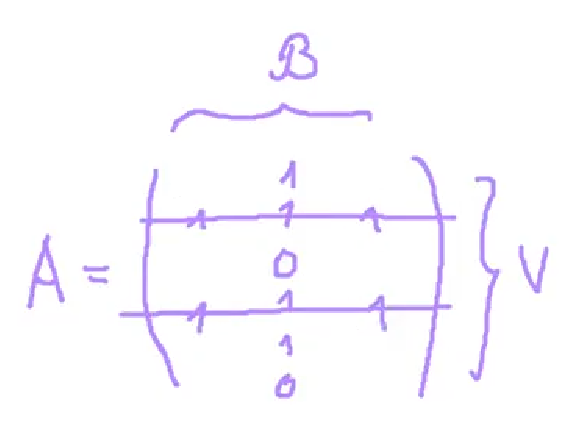
\includegraphics[scale=0.5]{bibd_0.eps}

	BIBD reprezentujeme pomoci matice incidence, pro niž platí:
	\begin{itemize}
		\item Z 2 axiomu, sloupcový součet je právě $k$.
		\item Z 3 axiomu, libovolné 2 sloupce mají jedničky na $\lambda$ společných pozicích.
			Neboli skalární součet je $\lambda$.
	\end{itemize}
\end{properties}

\begin{theorem}[Struktura BIBDu]\label{bibd_struct}
	Nechť $(V, \B)$ je $(v, k, \lambda)$-BIBD, pak
	\begin{enumerate}
		\item $\forall x \in V$ patří to $r = \frac{\lambda (v - 1)}{k - 1}$ bloků.
		\item $|\B| = \frac{\lambda v (v - 1)}{k(k - 1)}$
	\end{enumerate}
\end{theorem}
\begin{proof}
	1) ekvivalentně znamená, že řádkové součty matice se rovnají $r$.
	Zafixujeme libovolný prvek $x \in V$.
	Pak
	\[ r_x = |\{ B: x \in B \in \B \}| \]
	Spočítáme 2ma způsoby \# dvojic:
	\[ C = |\{ (y, B): x \ne y, x,y \in B \in \B \}| \]
	Na jedné straně je $r_x$ způsobů zvolit $B$ obsahující $x$ a $(k - 1)$ možnosti zvolit další prvek $y \in B$.

	Na druhou stranu, nejprve zvolíme $y$, což jde udělat $(v - 1)$ způsoby.
	Z axiomu 3 takové $x, y$ jsou ve $\lambda$ společných množinách.
	\[ r_x (k - 1) = C = (v - 1) \lambda \Rightarrow r_x = \frac{\lambda (v - 1)}{k - 1} \]
	Konečně, $x$ byl libovolný prvek, rovnost platí $\forall x \in V$.

	2) Jaký je součet všech prvků matice? Spočítáme po řádcích a po sloupcích
	\[ |\B| \cdot k = RS = SlS = v \cdot r = v \cdot \frac{\lambda (v - 1)}{k - 1} \Rightarrow |\B| = \frac{\lambda v (v - 1)}{k(k - 1)} \]
\end{proof}

\begin{properties}[Struktura BIBDu]\label{bibd_struct_c}
	Pokud pro parametry $\exists (v, k, \lambda)$-BIBD, tak:
	\begin{itemize}
		\item[D1] $\lambda(v - 1)$ je dělitelné $(k - 1)$.
		\item[D2] $\lambda \cdot v(v - 1)$ je dělitelné $k \cdot (k - 1)$.
		\item $r > \lambda$.
	\end{itemize}
\end{properties}
\begin{proof}
	Plyne hned z \cref{bibd_struct}, jelikož $r, |\B|$ jsou celá čísla.

	3 podmínka platí z předpokladu netriviality
	\[ v > k \Rightarrow (v - 1) > (k - 1) \Rightarrow \frac{r}{\lambda} = \frac{v - 1}{k - 1} > 1 \]
\end{proof}

\begin{example}
	Každá KPR(m) je $(m^2 + m + 1, m + 1, 1)$-BIBD.

	Každá KAR(m) je $(m^2, m, 1)$-BIBD.
\end{example}

\begin{theorem}[Wilson (1975) BD]
	\[ \forall k, \lambda \exists v_0: \forall v \geq v_0 \land \text{[D1] + [D2]} \Rightarrow \exists (v, k, \lambda)-BIBD \]
\end{theorem}

\begin{theorem}[Fisherová nerovnost]\label{fisher}
	Pokud $(V, \B)$ je $(v, k, \lambda)$-BIBD tak $|\B| \geq v$.
\end{theorem}
\begin{proof}
	Trik jako v mnoha důkazech přednášky LAK, mocnění matice incidence.
	Nechť $A$ je matice incidence BIBDu, pak
	\[ AA^T =
	\begin{pmatrix}
	r & \lambda & \ldots & \lambda \\
	\lambda & r & \ldots & \lambda \\
	\vdots & \vdots & \ddots & \vdots \\
	\lambda & \ldots & \lambda & r \\
	\end{pmatrix}
	= \lambda J + (r - \lambda)E
\]
	Spočítáme determinant pomoci vzorečku multilineární formy
	\[ det AA^{T} = (r - \lambda)^v + v \cdot \lambda \cdot (r - \lambda)^{v - 1} = (r - \lambda)^{v - 1}(r - \lambda + v \lambda) = (r - \lambda)^{v - 1}(v(\lambda - 1) + r) \]
	Dle \cref{bibd_struct_c} $r > \lambda \Rightarrow (r - \lambda)^{v - 1} > 0$.
	Dle axiomu BIBDu $\lambda - 1 \geq 0$ a $r > 0$.
	Takže i determinant je nenulový.
	Pak z LA
	\[ rank AA^{T} = v \leq rank A \leq |\B| \Rightarrow |\B| \geq v \]
\end{proof}

\begin{consequence}
	Pro každý BIBD $k \leq r$.
\end{consequence}
\begin{proof}
	\[ |\B| \cdot k = v \cdot r \land |\B| \geq v \Rightarrow k \leq r \]
\end{proof}

\subsection{Symetrické blokové schéma}

\begin{definition}[Symetrické blokové schéma]
	Blokové schéma se nazývá symetrické, pokud je počet jeho bloků roven počtu jeho prvků.
	\[ |\B| = v \]
	Neboli extremální případ Fisherové nerovnosti.
\end{definition}

\begin{theorem}[Ekvivalence BIBD]\label{bibd_equiv}
	Nechť $(V, \B)$ je množinový systém takový, že
	\begin{itemize}
		\item $|V| = v$
		\item $|\B| = b$
		\item $A \in \{ 0, 1\}^{v \times b}$ je matice incidence
		\item $k, \lambda, r = \frac{\lambda (v - 1)}{k - 1} \in \Z^+$
	\end{itemize}
	Pak $(V, \B)$ je $(v, k, \lambda)$-BIBD $\iff$:
	\begin{enumerate}
		\item $AA^T = \lambda J + (r - \lambda)E$
		\item $JA = kJ \iff$ sloupcový součet v matice A je $k$.
		\item $rank A = v$
	\end{enumerate}
\end{theorem}
\begin{proof}
	"$\Rightarrow$". Plyne z Fisherové nerovnosti \cref{fisher}.
	Z vlastnosti BIBDu \cref{bibd_struct_c} sloupcový součet v matice A je $k \Rightarrow JA = kJ$.

	"$\Leftarrow$". Ověříme axiomy:
	\begin{enumerate}
		\item TODO není axiom ale označení proměnné?
		\item $JA = kJ \Rightarrow$ sloupcový součet v matice A je $k \Rightarrow \forall B \in \B: |B| = k$
		\item z 1 podmínky plyne, že mimo diagonálu v $AA^T$ jsou $\lambda$.
			Což je skalární součin dvou libovolný řádku matice A.
		\item Nechť sporem $v = k$, tak $A = J$ a pro $v \geq 2$ by již neměla plnou hodnost.
			Spor s 3 podmínkou.
	\end{enumerate}

\end{proof}

\begin{theorem}[SBIBD ekvivalence]\label{sbibd_equiv}
	Nechť $(V, \B)$ je množinový systém takový, že $|V| = |\B| > 1$ a $A$ je matici incidence.
	Pak
	\begin{enumerate}
		\item Pokud je $(v, k, \lambda)$-SBIBD, tak
		\begin{enumerate}
			\item $AA^T = \lambda J + (k - \lambda)E \iff \forall x \in V$ patří do $k$ bloků, $\forall x \neq y \in V$ patří do $\lambda$ bloků.
			\item $A^TA = \lambda J + (k - \lambda)E$.
				Maticové násobení je skalárním součinem sloupců matice $A$, neboli se díváme na bloky.
				Rovnost ekvivalentně znamená, že na diagonále jsou velikosti bloku $k$ a mimo diagonálu průniky bloků $\lambda$.
				\[ \forall B \in \B: |B| = k, \forall B_1 \ne B_2 \in \B: |B_1 \cap B_2| = \lambda \]
			\item $JA = kJ \iff \forall$ prvek patří do $k$ bloků.
			\item $AJ = kJ$ násobíme charakteristický vektor s $\bar{1}$.
				Neboli $\forall B \in \B: |B| = k$.
			\item $A$ je regulární $\iff rank A = v$
		\end{enumerate}
		\item Nechť $A$ je regulární matice neboli platí e), potom pokud platí a) nebo b) $\Rightarrow (V, \B)$ je $(v, k, \lambda)$-SBIBD.
	\end{enumerate}
\end{theorem}
\begin{proof}
	Je vidět a) $\Rightarrow$ c) a b) $\Rightarrow$ d).

	Dle \cref{bibd_equiv} $(v, k, \lambda)$-SBIBD $\iff$ a), d), e).
	Potřebujeme zkontrolovat že b) je splněno.
	Ukážeme ale 1 a 2 dohromady pomoci implikace
	\begin{equation}\label{sbibd_equiv_eq}
		a), e) \Rightarrow b), d)
	\end{equation}

	2 je splněná taky, protože a), e) $\stackrel{\cref{sbibd_equiv_eq}}{\Rightarrow}$ b), d), c) znovu z \cref{bibd_equiv} $(V, \B)$ je $(v, k, \lambda)$-SBIBD.
	% cool symmetry usage
	Obraceně pokud platí b), e) pro $A \Rightarrow$ platí a), e) pro $A^T \Rightarrow$ a)-e) pro $A^T \Rightarrow$ a)-e) pro $A$.

	Začneme d).\\
	A regulární $\Rightarrow \exists A^{-1}$.
	Pak
	\[ A^{-1}AJ \stackrel{c)}{=} A^{-1}kJ = k A^{-1} J \stackrel{k \ne 0}{\Rightarrow} A^{-1}J = k^{-1} J \]
	Dal
	\[ JA^T = J^TA^T = (AJ)^T = (kJ)^T = k J \]
	Taky
	\[ A^T = A^{-1}AA^T \stackrel{a)}{=} = A^{-1}((k - \lambda)E + \lambda J) = (k - \lambda)A^{-1} + \lambda A^{-1}J = (k - \lambda)A^{-1} + \lambda k^{-1}J \]
	Z rovnosti usoudíme, že $k \ne \lambda$ protože jinak $A^T$ regulární $=c \cdot J$ která regulární není.
	Taky
	\[ JA^T = kJ = J ((k - \lambda)A^{-1} + \lambda k^{-1}J) = (k - \lambda)JA^{-1} + \lambda k^{-1}J^2 \]
	Jelikož $J \in \{ 0, 1 \}^{v \times v} \Rightarrow J^2 = vJ$ tak
	\[ JA^T = kJ = (k - \lambda)JA^{-1} + \lambda k^{-1} v J \Rightarrow (k - \lambda)JA^{-1} = (k - \lambda k^{-1} v)J \]
	Neboli
	\[ JA^{-1} = \frac{k - \lambda k^{-1} v}{k - \lambda} \Rightarrow J = JA^{-1}A = \frac{k - \lambda k^{-1} v}{k - \lambda}JA \]
	Označme $m = \frac{k - \lambda k^{-1} v}{k - \lambda}$, dal
	\[ J^2 = vJ = (mJA)J = (mJ) AJ = mJ kJ = mkJ^2 \Rightarrow mk = 1 \]
	Konečně máme d)
	\[ JA^{-1} = mJ = k^{-1}J \Rightarrow J = k^{-1}JA \Rightarrow JA = kJ \]

	b)
	\[ A^TA = ((k - \lambda)A^{-1} + \lambda k^{-1}J)A = (k - \lambda)E + \lambda k^{-1} k J = (k - \lambda)E + \lambda J \]
\end{proof}

\begin{consequence}[Duální SBIBD]
	Pokud $A$ je matice symetrického BIBDu $\Rightarrow A^T$ je matice duálního SBIBDu.
	Neboli
	\[ (V, \B)^{\ast} = (\B, V^{\ast}), V^{\ast} = \{ v^{\ast}: v \in V\}, v^{\ast} = \{ B: v \in B \in \B \} \]
\end{consequence}

\begin{definition}[Konstrukce blokových schémat ze symetrických]
	Pokud $(V, \B)$ je $(v, k, \lambda)$-BIBD, nechť $B_0$ je zafixovaný blok, definujme:
	\begin{enumerate}
		\item $(B_0, \{ B \cap B_0 : B \in \B \setminus \{ B_0 \} \})$ je $(k, \lambda, \lambda - 1)$-BIBD (odvozové schéma neboli v aj derived design).
		\item $(V \setminus B_0, \{ B \setminus B_0: B \in \B \setminus \{ B_0 \} \})$ je $(v - k, k - \lambda, \lambda)$-BIBD (zbytkové schéma neboli v aj residual design).
	\end{enumerate}
\end{definition}

\begin{example}[KPR vs KAR]\label{kpr_bibd}
	Každá konečná projektivní rovina je symetrický BIBD. Každá konečná afinní rovina je zbytkové schéma pro nějakou konečnou projektivní rovinu stejného řádu.
\end{example}
